% f2015zjw_q18_prism.tex — 2015 年高考数学·浙江卷·文科 第 18 题（三棱柱）
%
% 【来源】`.work/phase3-b18/source/2015浙江文.pdf`（SHA-256
%   a0e49283fb3d086029ec3c96de7e96cc6118365378ea0a24273c6f58285ec977），
%   第 2 页（合订本页 992）；内容对象 23。逐路径实测见
%   `.work/phase3-b18/figure-inventory.md`。
%
% 【坐标口径】源 PDF 用户空间（原点左下、y 向上）。本图本地坐标
%   (x, y) = (x_page − 259.718, y_page − 562.833)，1 单位 = 1 TeX pt。
%   路径坐标逐点照录内容流（含三次贝塞尔控制点）。
%
% 元素计数：12 条路径（8 实＋4 虚）＋7 个标签
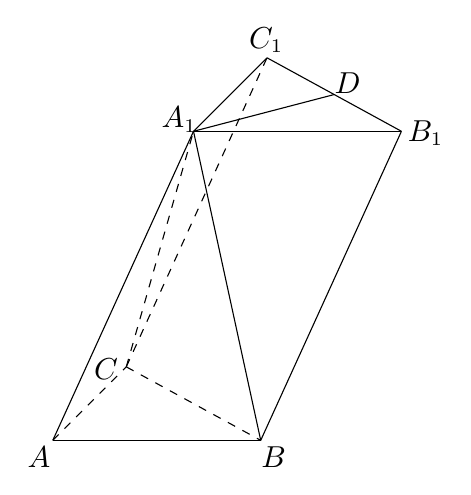
\begin{tikzpicture}[x=1pt, y=1pt,
    every node/.style={inner sep=0pt, font=\fontsize{10.5pt}{12.6pt}\selectfont}]
  \draw[line width=0.3985pt] (0.0000,0.0000)   (0.0000,0.0000)   -- (75.1352,0.0000);
  \draw[line width=0.3985pt] (75.1352,0.0000)   (75.1352,0.0000)   -- (50.8477,111.6752);
  \draw[line width=0.3985pt] (50.8477,111.6752)   (50.8477,111.6752)   -- (125.9829,111.6752);
  \draw[line width=0.3985pt] (125.9829,111.6752)   (125.9829,111.6752)   -- (77.4080,138.2355);
  \draw[line width=0.3985pt] (77.4080,138.2355)   (77.4080,138.2355)   -- (50.8477,111.6752);
  \draw[line width=0.3985pt] (75.1352,0.0000)   (75.1352,0.0000)   -- (125.9829,111.6752);
  \draw[line width=0.3985pt] (0.0000,0.0000)   (0.0000,0.0000)   -- (50.8477,111.6752);
  \draw[line width=0.3985pt] (101.6955,124.9553)   (101.6955,124.9553)   -- (50.8477,111.6752);
  \draw[line width=0.3985pt, dash pattern=on 2.98883pt off 2.98883pt, dash phase=0.0pt] (0.0000,0.0000)   (0.0000,0.0000)   -- (26.5603,26.5603);
  \draw[line width=0.3985pt, dash pattern=on 2.98883pt off 2.98883pt, dash phase=0.0pt] (26.5603,26.5603)   (26.5603,26.5603)   -- (77.4080,138.2355);
  \draw[line width=0.3985pt, dash pattern=on 2.98883pt off 2.98883pt, dash phase=0.0pt] (26.5603,26.5603)   (26.5603,26.5603)   -- (50.8477,111.6752);
  \draw[line width=0.3985pt, dash pattern=on 2.98883pt off 2.98883pt, dash phase=0.0pt] (26.5603,26.5603)   (26.5603,26.5603)   -- (75.1352,0.0000);

  \node[anchor=center] at (45.682,115.957) {$A_1$};  % 源中心 (305.40,678.79)
  \node[anchor=center] at (134.682,111.057) {$B_1$};  % 源中心 (394.40,673.89)
  \node[anchor=center] at (77.132,144.557) {$C_1$};  % 源中心 (336.85,707.39)
  \node[anchor=center] at (106.482,128.907) {$D$};  % 源中心 (366.20,691.74)
  \node[anchor=center] at (19.232,25.607) {$C$};  % 源中心 (278.95,588.44)
  \node[anchor=center] at (-4.968,-5.893) {$A$};  % 源中心 (254.75,556.94)
  \node[anchor=center] at (79.782,-5.893) {$B$};  % 源中心 (339.50,556.94)

\end{tikzpicture}
%
% 【自验结果】
%   探针：latexmk -pdfxe（待跑）。
